\documentclass[12pt]{article}
\usepackage{amsmath}
\usepackage{graphicx}
\usepackage{hyperref}
\usepackage[latin1]{inputenc}
\usepackage{enumitem}
\usepackage[margin=0.5in]{geometry}
\usepackage[LGRgreek]{mathastext}
\usepackage{framed}
\setlist[itemize]{noitemsep, topsep=0pt}
\title{10. Two sample}

\begin{document}

\begin{center}
\textbf{ILRST/STSCI 2100 Discussion 10: Chapter 11 Comparing Two Populations}
\end{center}

\noindent Reminders:
\begin{itemize}
\item Prelim 2 is in class next Wednesday!
\item Covers material up to and including chapter 10
\item You can bring a formula/note sheet, you will be given Table 2, 3, and 4.
\end{itemize}

\noindent \textbf{Comparing Two Sample Means:} \\
Assumes that both samples are randomly sampled, independent, and approximately normally distributed. We will be using the t-test Welch-Satterthwaite correction for calculating the degrees of freedom. \\

\noindent The null hypothesis is: $H_{0}: \mu_{1}-\mu_{2} = 0$\\
The alternative hypothesis is $H_{a}: \mu_{1} - \mu_{2} > 0$, could also be $<0$ or $\neq 0$. \\

\noindent T-statistic: $\cfrac{(\bar{X_{1}}-\bar{X_{2}})-(\mu_{1}-\mu_{2})}{\sqrt{\frac{s_{1}^{2}}{n_{1}}+\frac{s_{2}^{2}}{n_{2}}}}$ \\

\noindent This follows approximately the t-distribution with $df = \cfrac{(\frac{s_{1}^{2}}{n_{1}}+\frac{s_{2}^{2}}{n_{2}})^{2}}{\frac{s_{1}^{4}}{n_{1}^{2}(n_{1}-1)}+\frac{s_{2}^{4}}{n_{2}^{2}(n_{2}-1)}}$ \\

\noindent Then you can find the p-value and make a decision to the hypothesis test\\

\noindent Confidence interval: $(\bar{X_{1}}-\bar{X_{2}}) \pm t_{\frac{\alpha}{2}} \sqrt{\frac{s_{1}^{2}}{n_{1}}+\frac{s_{2}^{2}}{n_{2}}}$ \\


\noindent \textbf{Paired-sample t-test}\\
We can compute differences for each pair of observations, and then compute the mean and standard deviation using the differences. Note that when looking at these samples, these are \textbf{not} independent.\\
\noindent Ex.
\begin{itemize}[noitemsep,nolistsep]
\item Pre-test and post-test scores after online tutorial
\item Comparing fertilizer vs no fertilizer on grass growth on the same patch of grass\\
\end{itemize}
Assuming that the population is approximately normal, or if $n>30$, we can calculate a test statistic that follows the t-distribution with $df = n-1$. Note that $n$ is the number of pairs. \\

\noindent The null hypothesis would be: $H_{0}: \mu_{D}=0$\\

\noindent And the alternative hypothesis could be: $H_{a}: \mu_{D} >0$, could also be $<0$ or $\neq 0$\\

Use the t-test, and calculate the t statistic:\\
\begin{center}
$t_{obs} = \cfrac{\bar{D}-\mu_{D}}{SD_{D}/\sqrt{n}}$, where $SD_{D} = \sqrt{\frac{1}{n-1}\sum(D_{i}-\bar{D})^{2}}$
\end{center}
$\cfrac{SD_{D}}{\sqrt{n}}$ is also called the standard error. \\

\noindent Confidence interval = $\bar{D} \pm t_{\alpha/2}\cfrac{SD_{D}}{\sqrt{n}}$ \\ 
\newpage
\noindent \textbf{Comparing Two Population Proportions:}\\
You must first check that the sample sizes for each population is sufficiently large by making sure $n_{1}*p_{1}$, $n_{1}*(1-p_{1})$,$n_{2}*p_{2}$, and $n_{2}*(1-p_{2})$ are all greater than 10.\\
The null hypothesis is: $H_{0}: p_{1}-p_{2}=0$\\
The alternative would be: $H_{a}: p_{1}-p_{2} > 0$, can also be $<0$ or $\neq 0$\\
  
\noindent The test statistic would be:\\
$Z=\cfrac{\hat{p_{1}}-\hat{p_{2}}}{\sqrt{\hat{p_{c}}(1-\hat{p_{c}})(\cfrac{1}{n_{1}}+\cfrac{1}{n_{2}})}}$, where $\hat{p}_{c} = \frac{X_{1}+X_{2}}{n_{1}+n_{2}}$, where $X_{1}$ and $X_{2}$ are number of success in population 1 and 2, respectively. \\

\noindent Find p-value and make a decision.\\

\noindent \textbf{Examples:}

\begin{enumerate}
\item
A researcher is interested in comparing the average fish length (cm) in two lakes in a fishing community. People tend to fish in Lake A, whereas very few people fish in Lake B. Run a hypothesis test comparing two sample means (assume population variances are not equal). 

\begin{center}
\begin{tabular}{ |c|c|c|c| } 
 \hline
 Sample & n & $\bar{x}$ & $s^{2}$ \\ 
 Lake A & 32 & 15 & 2 \\ 
 Lake B & 34 & 20 & 4 \\ 
 \hline
\end{tabular}
\end{center}

\vspace{25 mm}

\item
(modified from: http://stattrek.com/hypothesis-test/paired-means.aspx?tutorial=ap) \\
44 students are randomly selected from a school and divided into 22 matched pairs, each pair having an equal GPA. One student in each pair was given a special online tutorial on a concept in statistics. Then, all students were tested. Conduct a hypothesis test to determine if the online tutorial helped students better understand the concept. Use $\alpha=0.05$ and assume mean differences are normally distributed. Test results are summarized below.
\begin{center}
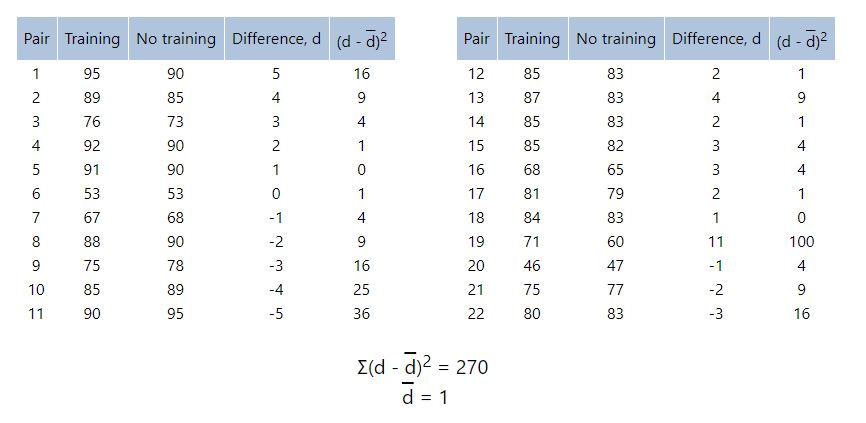
\includegraphics[scale = 1.2]{samplepair}
\end{center}

\vspace{25mm}

\item
Calculate a 95\% confidence interval for the data in problem 2. Is your answer consistent with the decision in problem 2? \\

\vspace{25mm}

\end{enumerate}

\newpage

\begin{framed}

Assume that both samples are randomly sampled, independent and check samples sizes $(n_{1} = 32, n_{2}=34)$ are greater than 30. \\

\textbf{Step 1:} Define $H_{0}$\\
$H_{0}: \mu_{1} - \mu_{2} = 0$\\
(Be sure to use the population parameter $\mu$ in hypotheses) \\

\textbf{Step 2:} Define $H_{1}$\\
$H_{1}: \mu_{1} - \mu_{2} \neq 0$\\
(This is two-sided test)\\


\textbf{Step 3:} Calculate test statistic
\begin{align*}
t_{obs} &= \cfrac{(15-20)-0}{\sqrt{\cfrac{2}{32}+\cfrac{4}{34}}} \\
&= -11.7 
\end{align*}

Calculate d.f
$df = \frac{\left(\cfrac{2}{32}+\cfrac{4}{34}\right)^{2}}{\cfrac{2^{2}}{32^{2}(32-1)}+\cfrac{4^{2}}{34^{2}(34-1)}} = 59.5$\\
  
\textbf{Step 4:} Find p-value \\
Since this is a two-sided test:\\
\begin{eqnarray*}
P-value &=& 2*P(T > |t_{obs}|) \\
&=& 2*P(T > |-11.7|) \\
&=& \approx 0
\end{eqnarray*}

\textbf{Step 5:} Decision \\
The observed t-statistic is in the rejection region and p-value $< \alpha$ so we reject the null hypothesis. We conclude that there is a significant difference between fish lengths in Lake A and Lake B.\\
\end{framed}

\begin{framed}
\textbf{Step 1:} Define $H_{0}$ \\
$H_{0}: \mu_{D} = 0$\\

\textbf{Step 2:} Define $H_{1}$ \\
$H_{0}: \mu_{D} \neq 0$\\
(Two-sided test)\\

\textbf{Step 3:} Calculate test statistic \\
Standard deviation of differences: $SD_{D} = \sqrt{\cfrac{\sum(d_{i}-\bar{d})^{2}}{n-1}} = \sqrt{\frac{270}{(22-1)}} = 3.586 $ \\

$t_{obs} = \cfrac{1-0}{\cfrac{3.586}{\sqrt{22}}} = 1.307$ \\

\textbf{Step 4:} Find p-value \\

p-value = $2*P(T > |t_{obs}|) = 2*P(T>|1.307|)$ \\

$df= n - 1 = 22 - 1$ (n is the number of pairs)
If you look in Table 4, you'll see that the central area is $<$80\%, meaning that the area in the two tails is greater than 20\%. Area in the two tails is the p-value, so the p-value is greater than 20\%.\\

\textbf{Step 5:} Decision \\ 
At $\alpha = 0.05$, p-value $> \alpha$ so we fail to reject the null hypothesis. There is no significant difference in performance on a test between those who have completed an online tutorial and those who have not. \\

\end{framed}

\begin{framed}
\noindent Confidence interval = $\bar{D} \pm t_{\alpha/2}\cfrac{SD_{D}}{\sqrt{n}}$ \\

\noindent 95\% confidence interval means $\alpha = 0.05$ so $t_{\alpha/2} = 2.08$ \\

\noindent From problem 2, $SD_{D} = 3.586$ \\

\noindent So the confidence interval is: $1 \pm 2.08*\cfrac{3.586}{\sqrt{21}} = (-6.28, 2.63)$ \\

Since 0 is included in the confidence interval, we conclude that the mean difference between the two groups is zero. So our results match the hypothesis test. 
\end{framed}


\end{document}
